%%%%%%%%%%%%%%%%%%%%%%%%%%%%%%%%%%%%%%%%%%%%%%
%                insertmeeting
% 1) Title (something creative & funny?)
% 2) Date (MM/DD/YYYY)
% 3) Location (ex. Hagerty High School)
% 4) People/Committees Present 
% 5) Picture 
% 6) Start Time & Stop Time (ex. 12:30AM to 4:30PM)
%%%%%%%%%%%%%%%%%%%%%%%%%%%%%%%%%%%%%%%%%%%%%%
\insertmeeting 
	{Speed vs. Velocity} 
	{01/04/22} 
	{Hagerty High School}
	{Anouska, James, Ritam, Samantha}
	{Images/RobotPics/robot.jpg}
	{2:30 - 4:30}
	
\hhscommittee{Software}
\noindent\hfil\rule{\textwidth}{.4pt}\hfil
\subsubsection*{Goals}
\begin{itemize}
    \item Develop a system to convert wheel velocities to a robot velocity.

\end{itemize} 

\noindent\hfil\rule{\textwidth}{.4pt}\hfil

\subsubsection*{Accomplishments}
We created a function in Kotlin named "wheelToRobotVelocities" that takes in wheelVelocities and steeringAngle as arguments. The function finds the left and right wheel velocities, then converts them to a robot velocity. The derviation of the formula can be found in the attached picture. 


\begin{figure}[htp]
\centering
\includegraphics[width=0.95\textwidth, angle=0]{Meetings/January/01-04-22/SteeringAngletoHeadingFormula - Big Boik.JPG}
\caption{Deriving our tricycle kinematic formulas}
\label{fig:010422_1}
\end{figure}

	
\hhscommittee{Hardware}
\noindent\hfil\rule{\textwidth}{.4pt}\hfil
\subsubsection*{Goals}
\begin{itemize}
    \item Build and test smaller roller intake
	\item Make sure robot is ready for competition


\end{itemize} 

\noindent\hfil\rule{\textwidth}{.4pt}\hfil

\subsubsection*{Accomplishments}
Working fast to get our new intake working and on the robot in time, we got our new intake from the nylon 3D printer and started building the new intake right away (Figure \ref{fig:010422_2}). Because we were hoping to make this intake the final version we use at competition, we used  surgical tubing instead of rubber bands. To get the surgical tubing around our roller, we tied one side of the surgical tubing shut, and used compressed air to blow the tube up to size. Then, we pushed the tubing over the roller, releasing the air from the tube once it completely covered the roller. The end product gave us the roller with the surgical tubing wrapped tightly around it. From there we started putting together the rest of the intake in a similar process to how we built the other roller intake. This time however, we used less bearings to reduce weight and the servo was directly connected to the side of the intake. We used standoffs to place the servo at the right distance from the intake. Because we also wanted to be able to sense when we have a game element, we screwed a color sensor to the top of the roller arm, where it can look through a hole to sense if anything has been picked up. After Screwing a small sheet metal funnel that should make up for the smaller size of the intake, the intake was complete (Figure \ref{fig:010422_3}). 
Although we changed the main design of the intake, we expected it to work very similarly as it had the same basic features like a roller, o-ring belts, and a pivoting coaxial roller arm (Figure \ref{fig:010422_4}). Despite our expectations however, the intake didn’t grab the blocks quite as quickly as our first version, but it still was considerably faster than our old grabber intake. We suspect the reason for not grabbing as fast as our first roller design has more to do with how it was powered than with any design elements. We tested the first design with a drill and this one is powered with a superspeed servo, two power sources that are drastically different in power. Still feeling optimistic about the design, we kept testing, but found a fatal flaw of the design. The pivoting roller arm worked well while level and on the ground, but when the arm swung backwards to score and turns the intake upside down, the intake would fling whatever element it was holding, an infraction that would give us a minor penalty. This is because when the arm swings around and turns the intake upside down, the centripetal force as well as the added force of gravity forced the roller arm to pivot and release the element. Although the obvious solution would be to increase the tension holding the roller down, when we tested this out, we found that more tension made it very difficult to pick up elements, especially balls, because the roller arm no longer pivots to the correct height as easily. Unsure how to fix the issue, we faced the option of using an intake that doesn’t work properly or going back once again to our old grabber design. Feeling somewhat dejected and unable to fix the new intake, we decided to return to the grabber intake and make some modifications to fix any of its remaining problems, still hoping to redesign and build a better intake before meet 4.
The modifications we made were simple but should fix the remaining problems with the intake. At meet 2, we still observed some issues with accidentally picking up 2 blocks at once, so we decided to combat this in 2 ways. The first was to reduce the length of the fiberglass plate by .25 inches. We did this so that if 2 blocks are grabbed, when we pivot the arm, one will be held loosely at the bottom and will be left behind. The other modification is to once again change the rubber placement, but this time to have one thin strip down the middle instead of two on the outside(Figure \ref{fig:010422_5}). This will help us with only grabbing one block by only having enough space to clamp down on one at a time if they come into the intake side by side. Having a lower surface area of rubber will also give the rubber more squish, hopefully holding the elements in tighter. When testing these adjustments, we found that they worked surprisingly well for such simple changes. We couldn’t even pick up 2 blocks when we tried! Although the roler intake didn't work out, we are still feeling optimistic for the upcoming meet thanks to these simple modifications. We also feel more inspired than ever to fix the roller intake so that we can use it in meet 4.

\begin{figure}[ht]
\centering
\begin{minipage}[b]{.48\textwidth}
  \centering
  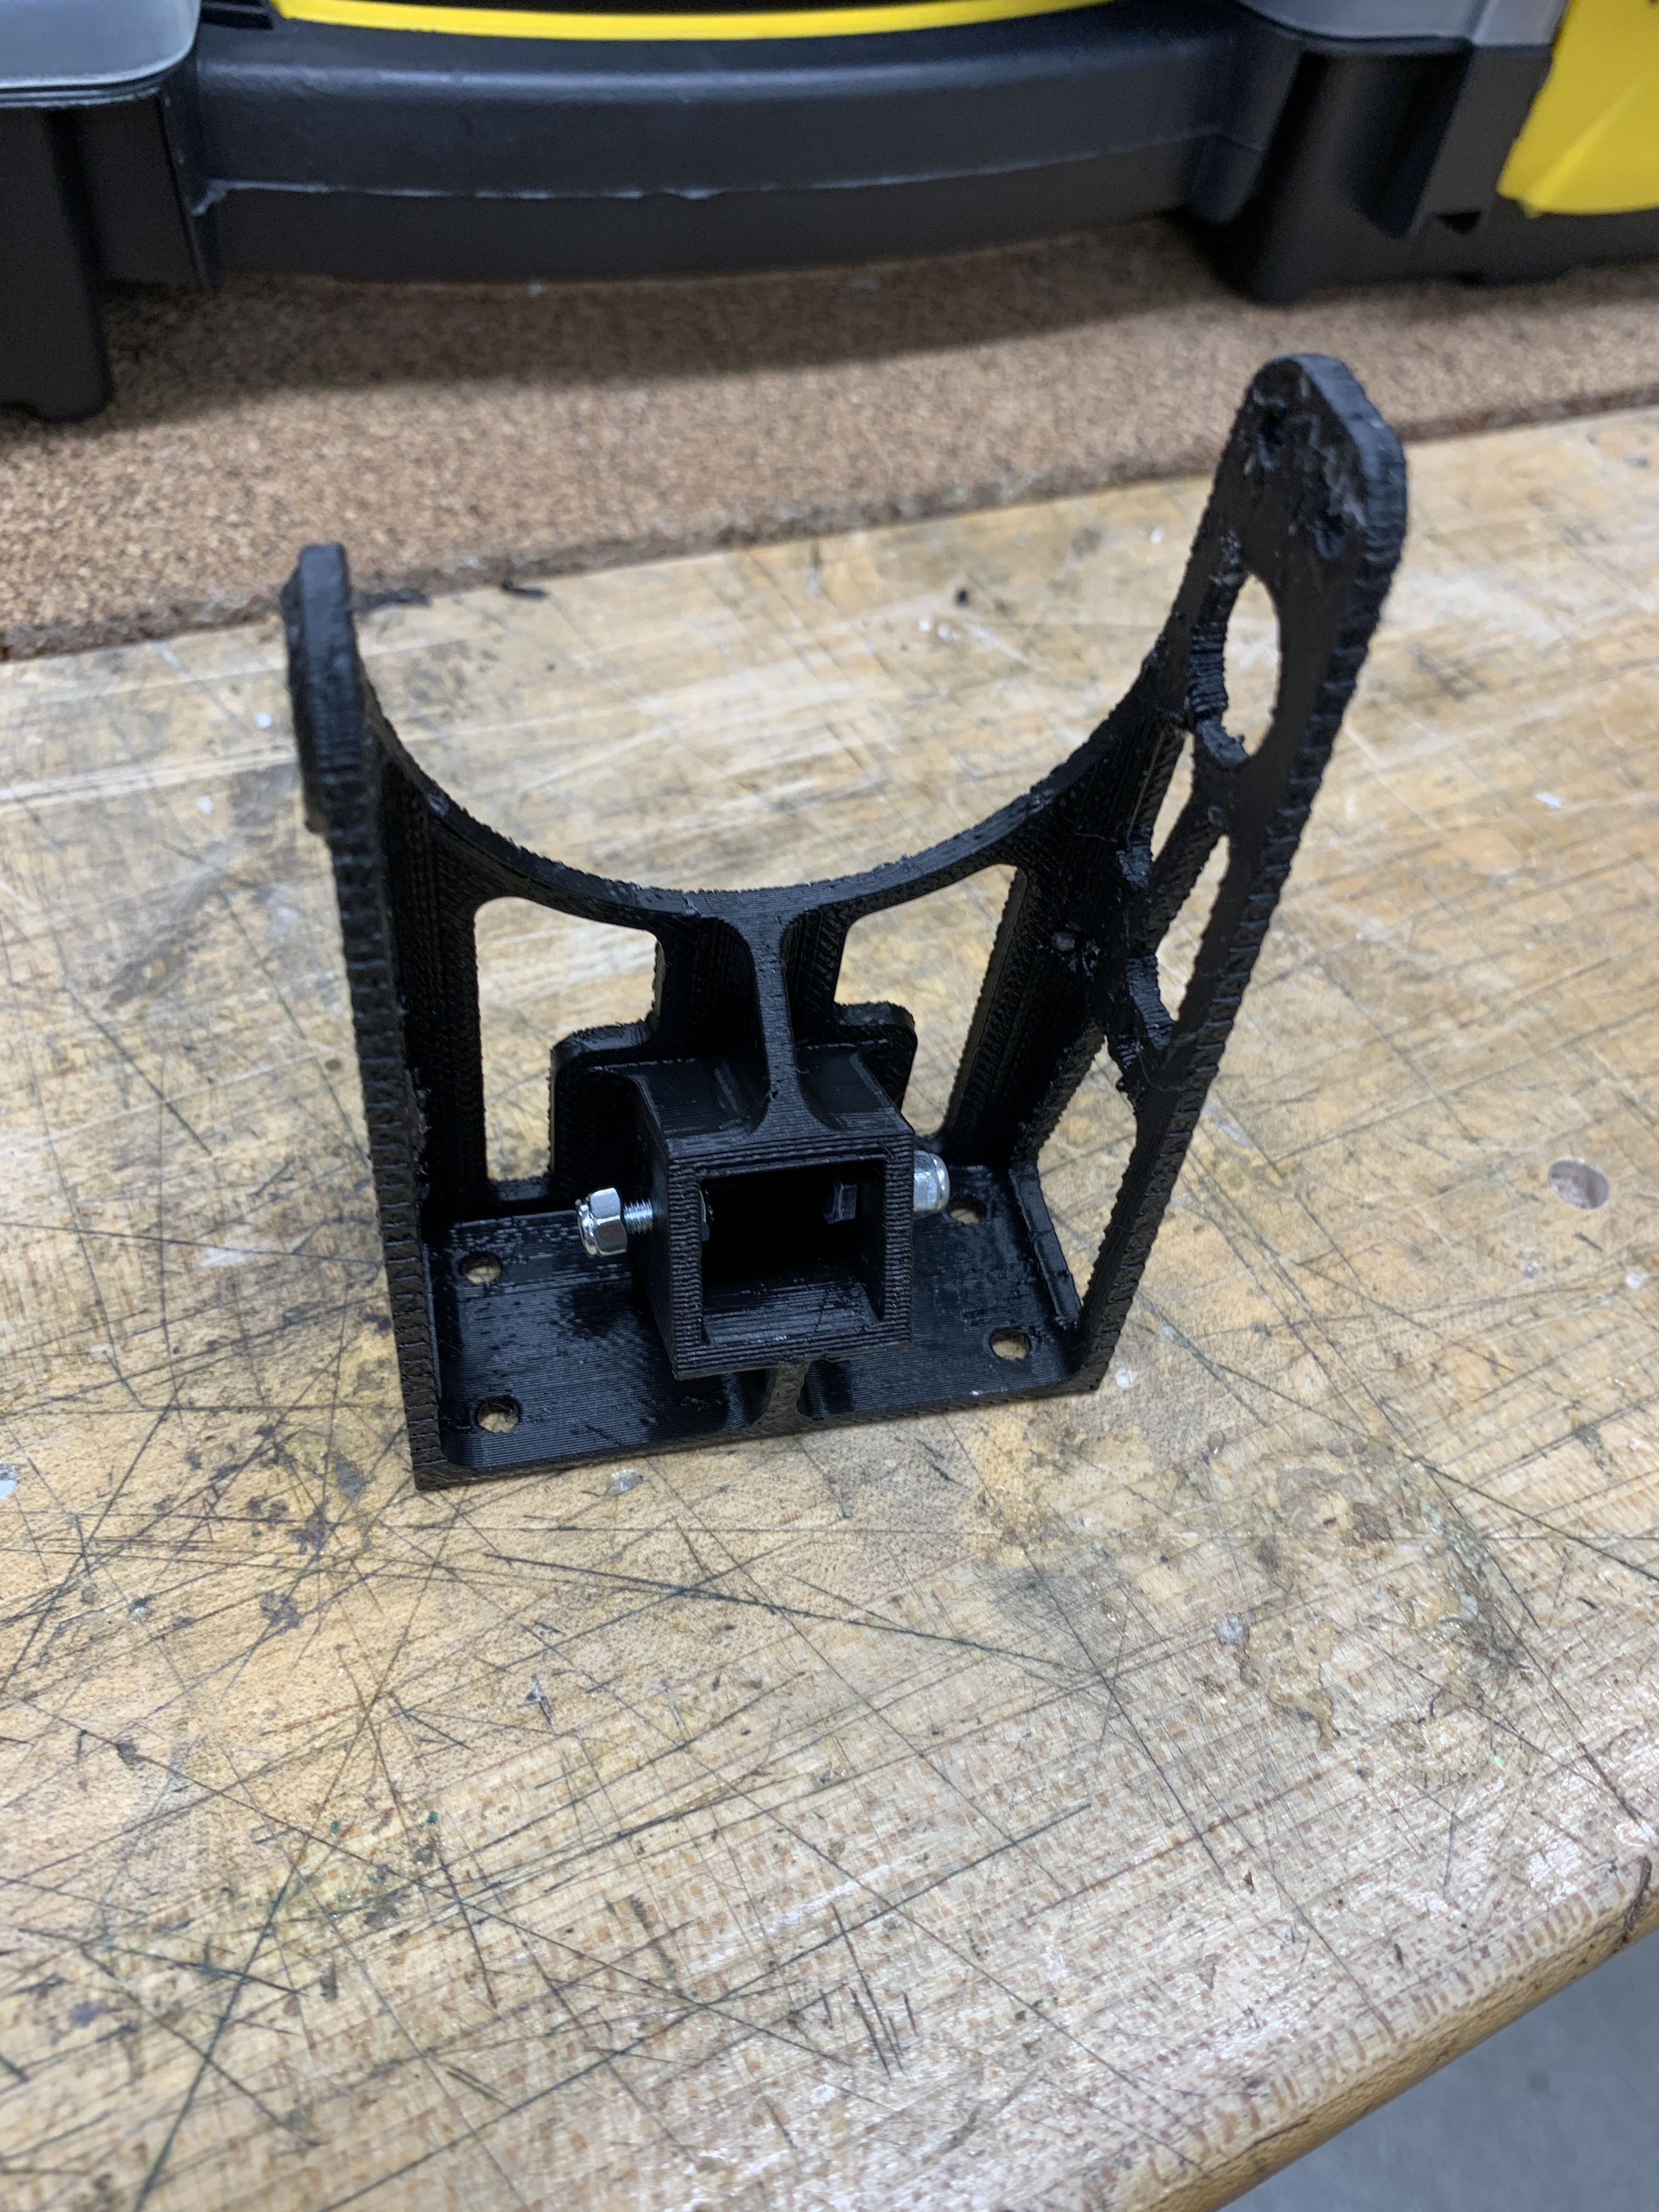
\includegraphics[width=0.95\textwidth]{Meetings/January/01-04-22/1-4-22_Hardware_Figure1 - Nathan Forrer.JPG}
  \caption{New 3D printed intake}
  \label{fig:010422_2}
\end{minipage}%
\hfill%
\begin{minipage}[b]{.48\textwidth}
  \centering
  \includegraphics[width=0.95\textwidth]{Meetings/January/01-04-22/1-4-22_Hardware_Figure2 - Nathan Forrer.JPG}
  \caption{Complete intake}
  \label{fig:010422_3}
\end{minipage}
\end{figure}

\begin{figure}[ht]
\centering
\begin{minipage}[b]{.48\textwidth}
  \centering
  \includegraphics[width=0.95\textwidth]{Meetings/January/01-04-22/1-4-22_Hardware_Figure3 - Nathan Forrer.JPG}
  \caption{New intake}
  \label{fig:010422_4}
\end{minipage}%
\hfill%
\begin{minipage}[b]{.48\textwidth}
  \centering
  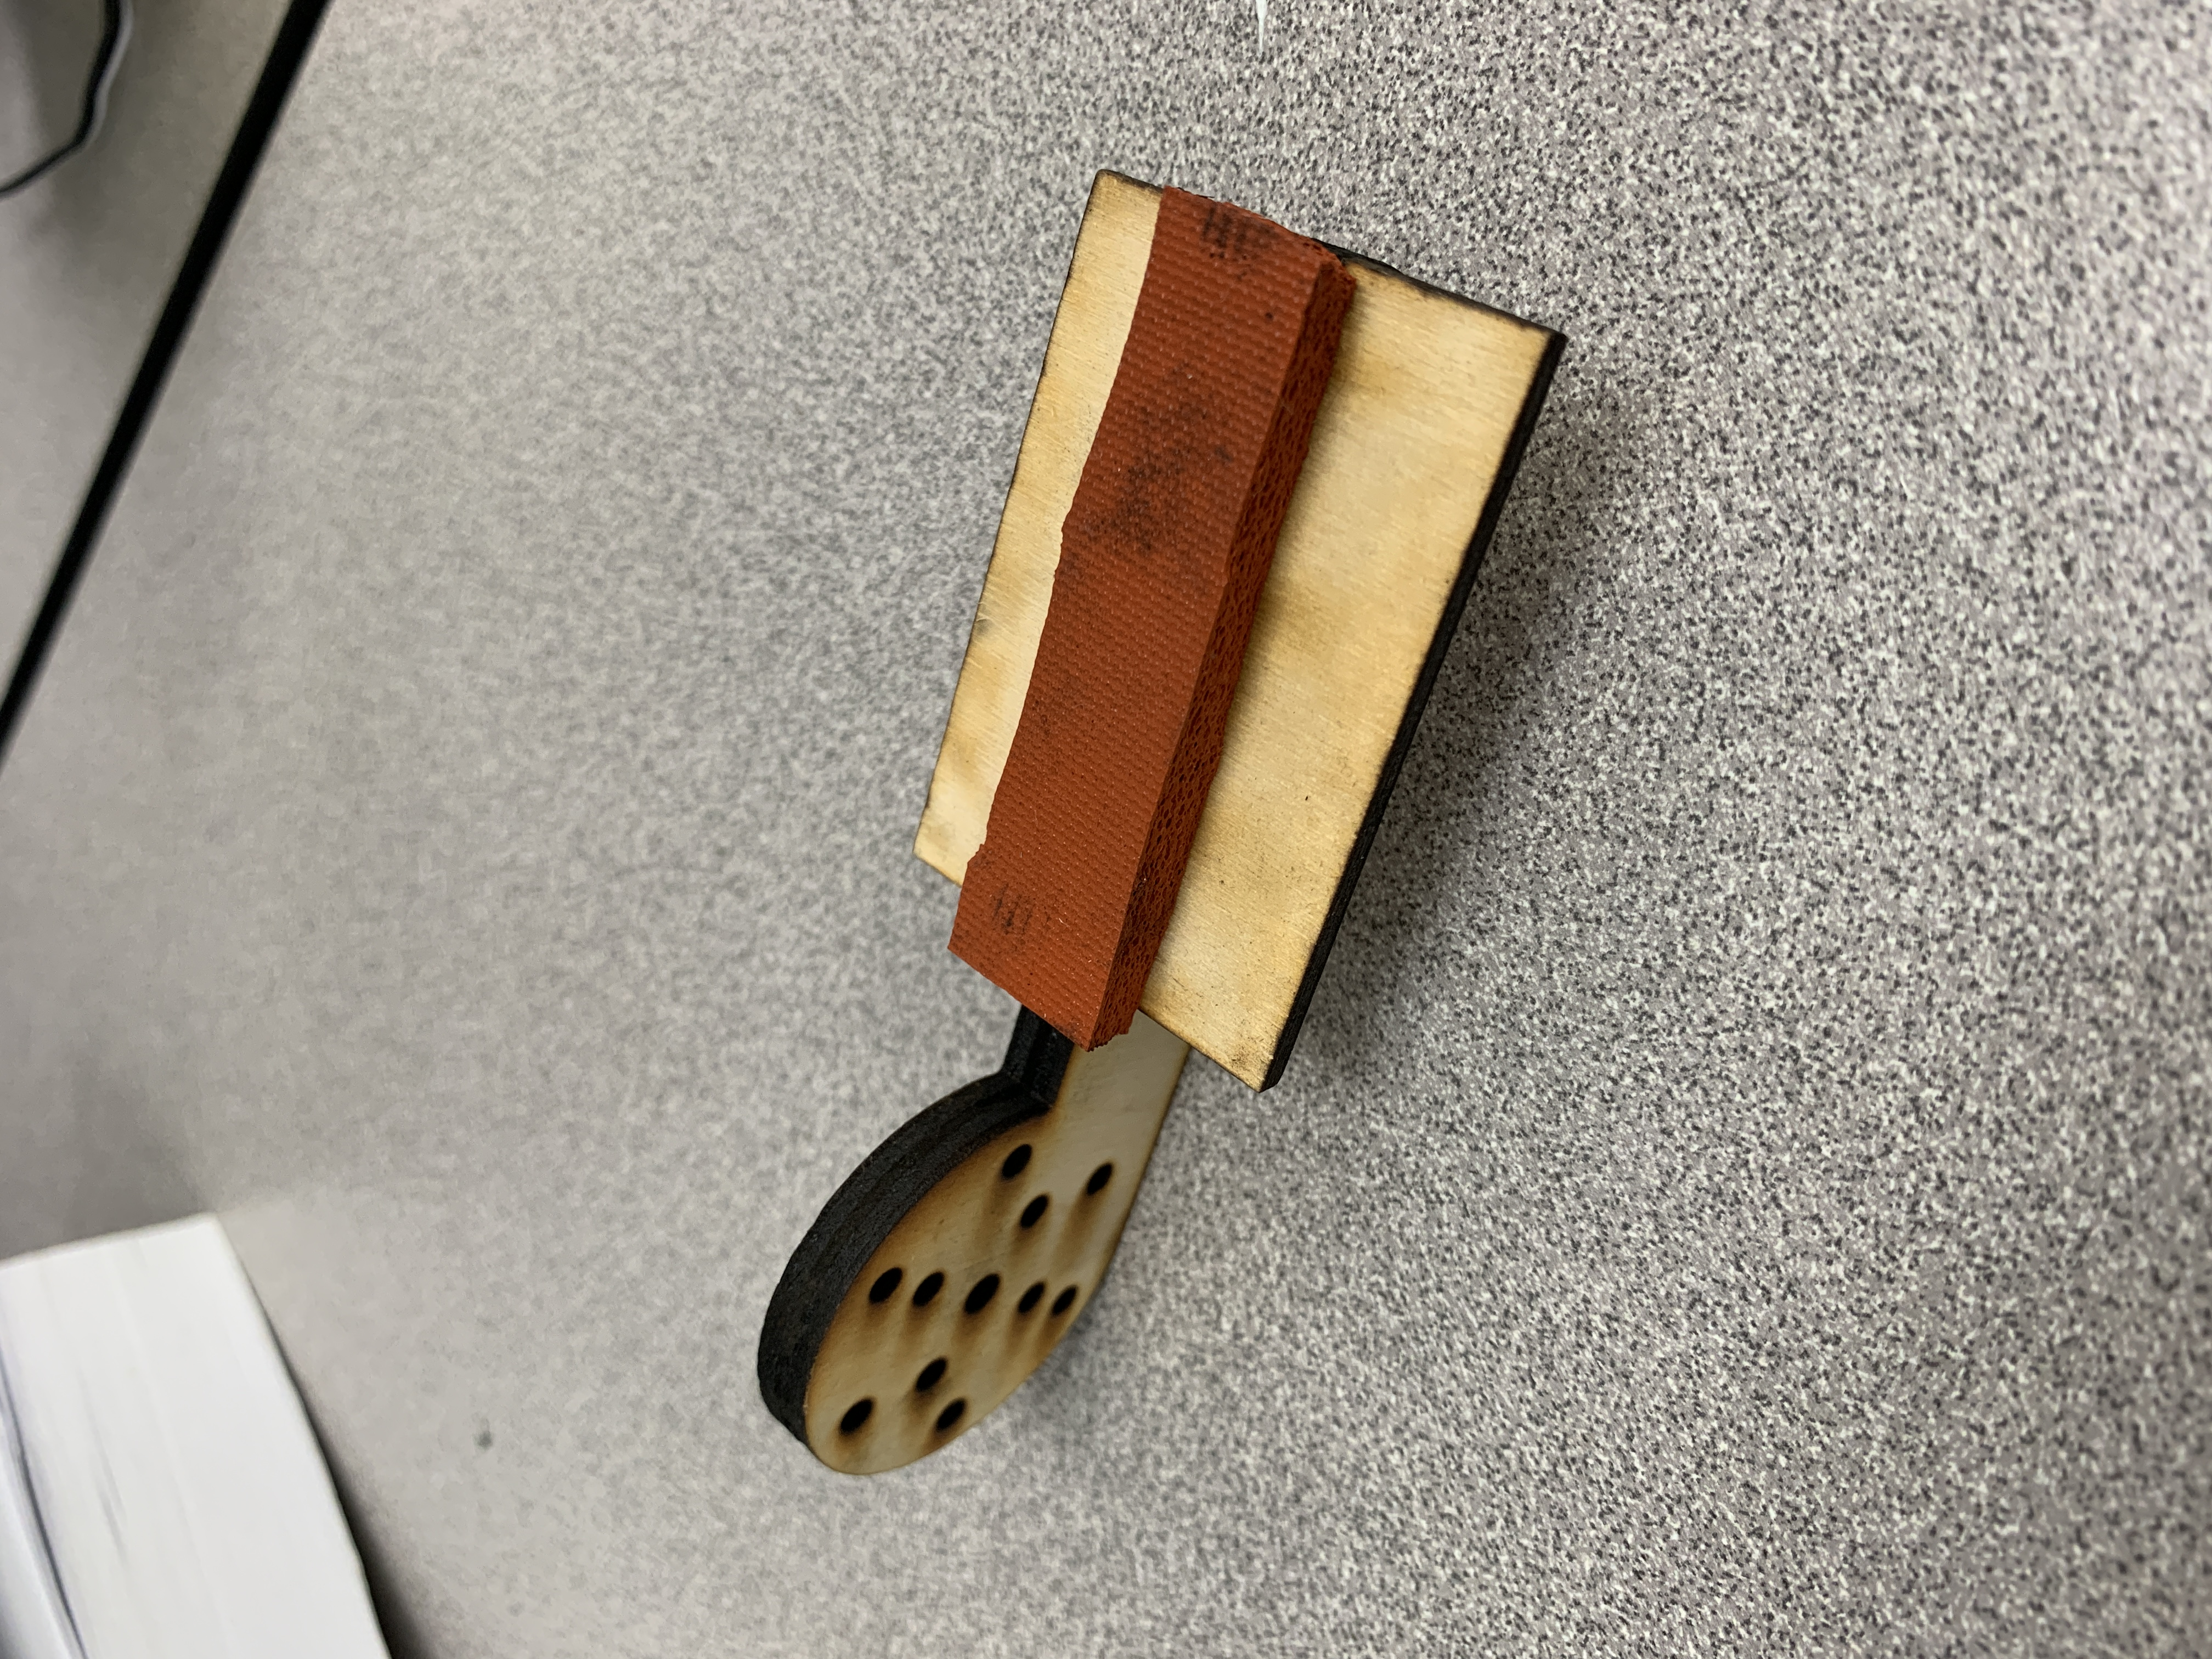
\includegraphics[width=0.95\textwidth]{Meetings/January/01-04-22/1-4-22_Hardware_Figure4 - Nathan Forrer.JPG}
  \caption{Modified rubber placement}
  \label{fig:010422_5}
\end{minipage}
\end{figure}

\whatsnext{
\begin{itemize}
    \item Improve reliability of the system.
    \item Give software time to finish autonomous
	\item Fix any hardware issues that arise before meet 3
 
\end{itemize} 
}

